\documentclass[a4paper,12pt]{report}
\usepackage[utf8]{inputenc}
\usepackage[francais]{babel}
\usepackage{fancyhdr}
\usepackage{graphicx}
\usepackage{tikz}
\usetikzlibrary{calc}
\usepackage{listings}
\usepackage{xcolor}
\definecolor{grey}{rgb}{0.9,0.9,0.9}
\usepackage{titlesec}
\usepackage{verbatim}
\usepackage{listings}
\usepackage{textcomp}
\usepackage{hyperref}
\usepackage{longtable}
\usepackage{colortbl}
\usepackage{amssymb}

\frenchbsetup{StandardLists=true}
\newcommand{\marge}{18mm}
\usepackage[left=\marge,right=\marge,top=\marge,bottom=\marge]{geometry}
\pagestyle{fancy}
\setlength{\headheight}{14pt}
\chead{
   Badache Yassine
  \hspace{13em}
  Sujet 70: Serveur de jeux au tour par tour}
\renewcommand{\headrulewidth}{1pt}
\linespread{1}
\setlength{\columnseprule}{0.2pt}
\definecolor{javakeyword}{rgb}{0,0,0.5}
\definecolor{javastring}{rgb}{0,0.5,0}
\definecolor{javacomment}{rgb}{0.5,0.5,0.5}
\lstdefinestyle{java}{
   language=Java, basicstyle=\footnotesize,       % the size of the fonts that are used for the code
  numbers=left,                   % where to put the line-numbers
  numberstyle=\tiny\color{gray},  % the style that is used for the line-numbers
  stepnumber=1,                   % the step between two line-numbers. If it's 1, each line
                                  % will be numbered
  numbersep=5pt,                  % how far the line-numbers are from the code
  backgroundcolor=\color{white},  % choose the background color. You must add \usepackage{color}
  showspaces=false,               % show spaces adding particular underscores
  showstringspaces=false,         % underline spaces within strings
  showtabs=false,                 % show tabs within strings adding particular underscores
  frame=single,                   % adds a frame around the code
  rulecolor=\color{black},        % if not set, the frame-color may be changed on line-breaks within not-black text (e.g. commens (green here))
  tabsize=2,                      % sets default tabsize to 2 spaces
  captionpos=b,                   % sets the caption-position to bottom
  breaklines=true,                % sets automatic line breaking
  breakatwhitespace=false,        % sets if automatic breaks should only happen at whitespace
  title=\lstname,                 % show the filename of files included with \lstinputlisting;
   stringstyle=\color{javastring},
   keywordstyle=\color{javakeyword}\ttfamily\textbf,
   commentstyle=\color{javacomment}\ttfamily\textit
 }
 
 \bibliographystyle{plain}
 \frenchbsetup{StandardLists=true}
 
 %%%%%%%%%%%%%%%%%%%%%%%%%%%%%%%%%%%%%%% PDF INFO 
 %%%%%%%%%%%%%%%%%%%%%%%%%%%%%%%%%%%%%%%%%%%%%%%%
 \hypersetup{
 	pdfauthor   = {Yassine Badache},
 	pdftitle    = {Rapport de PJI (Projet individuel)},
 	pdfsubject  = {Serveur de jeux au tour par tour},
 	pdfkeywords = {Lille Serveur Jeux Yassine Badache PJI},
 	pdfcreator  = {PDFLaTeX},
 	pdfproducer = {PDFLaTeX}
 }
 %%%%%%%%%%%%%%%%%%%%%%%%%%%%%%%%%%%%%%%%%%%%%%%%
 
\author{Yassine Badache}
\title{}
\titleformat{\chapter}[hang]{\bf\huge}{\thechapter}{2pc}{}
\begin{document}
	
	\makeatletter
\begin{titlepage}
\centering
{\LARGE \textbf{\textsc{Projet Individuel}}}\\
\vspace{20em}
{\LARGE \textsc{Sujet 70: Serveur de jeux au tour par tour
}}\\


\vspace{6em}
{\LARGE Etudiant: Yassine Badache\\
	\vspace{2em}
		Encadrants: Yoann DUFRESNE, Gauvin MARQUET}\\


\vspace{15em}

\begin{tikzpicture}[remember picture,overlay]

\node [below left,xshift=-1cm, yshift=4cm] at (current page.south east){
\includegraphics[scale=0.6]{images/ustl1.jpg}};

\end{tikzpicture}
\end{titlepage}
\makeatother

\sloppy
	\input{thanks.tex}

	\tableofcontents	
	\newpage
	\setcounter{page}{1}
% Début de document

	\chapter{Introduction}

	L'an dernier, deux étudiants en Master 1 Informatique ont développé un \textit{framework} permettant de développer, à l'aide d'automates, des jeux au tour par tour. Les jeux ainsi implémentés peuvent héberger une partie de manière indépendante, contenant les protocoles de communication entre elle-même et le client.
	\\
	
	Le but principal de ce PJI était de concevoir un composant logiciel permettant d'accéder aux différents jeux implémentés, et de les instancier par ce biais. Ceci permettrait alors un accès simplifié aux jeux développés et une centralisation des ressources nécessaires à son bon fonctionnement.
	\\
	
	Au-delà de l'accès public aux ressources, c'est notamment dans une vision plus 'interne' qu'a été proposé ce projet individuel. En effet, l'aboutissement final de ce composant logiciel serait d'héberger des intelligences artificelles, s'affrontant sur les supports développés via le \textit{framework} de l'an dernier.
	\\
	\chapter{Conception}

Le programme développé ici est supposé répondre à un besoin bien précis, c'est-à-dire l'accessibilité d'une ressource bien définie et son utilisation, que ce soit par un utilisateur humain ou par une intelligence artificielle développée spécifiquement pour le jeu souhaité. La première partie de ce projet a donc été dédiée à la conception de ce projet par les besoins d'un utilisateur quel qu'il soit.\\

Ci-dessous sont détaillés les scénarios d'usage du logiciel, ainsi que leurs diagrammes de séquence associés. C'est l'ensemble de ces éléments qui nous a permis par la suite de cerner le cœur de ce qui est attendu à la fin de ce sujet.\\


\begin{figure}[!ht]
	\center
	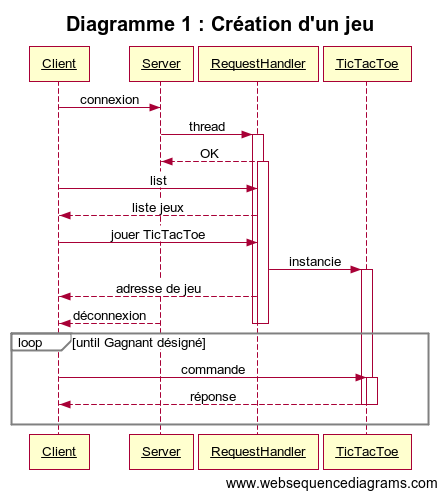
\includegraphics[scale=0.5]{images/sequence/diagramme_scenario1.png}
	\caption{Le premier cas d'utilisation, basique}
\end{figure}

% Fin du contenu	
	
	
\end{document}